% Options for packages loaded elsewhere
\PassOptionsToPackage{unicode}{hyperref}
\PassOptionsToPackage{hyphens}{url}
%
\documentclass[
]{article}
\usepackage{lmodern}
\usepackage{amssymb,amsmath}
\usepackage{ifxetex,ifluatex}
\ifnum 0\ifxetex 1\fi\ifluatex 1\fi=0 % if pdftex
  \usepackage[T1]{fontenc}
  \usepackage[utf8]{inputenc}
  \usepackage{textcomp} % provide euro and other symbols
\else % if luatex or xetex
  \usepackage{unicode-math}
  \defaultfontfeatures{Scale=MatchLowercase}
  \defaultfontfeatures[\rmfamily]{Ligatures=TeX,Scale=1}
\fi
% Use upquote if available, for straight quotes in verbatim environments
\IfFileExists{upquote.sty}{\usepackage{upquote}}{}
\IfFileExists{microtype.sty}{% use microtype if available
  \usepackage[]{microtype}
  \UseMicrotypeSet[protrusion]{basicmath} % disable protrusion for tt fonts
}{}
\makeatletter
\@ifundefined{KOMAClassName}{% if non-KOMA class
  \IfFileExists{parskip.sty}{%
    \usepackage{parskip}
  }{% else
    \setlength{\parindent}{0pt}
    \setlength{\parskip}{6pt plus 2pt minus 1pt}}
}{% if KOMA class
  \KOMAoptions{parskip=half}}
\makeatother
\usepackage{xcolor}
\IfFileExists{xurl.sty}{\usepackage{xurl}}{} % add URL line breaks if available
\IfFileExists{bookmark.sty}{\usepackage{bookmark}}{\usepackage{hyperref}}
\hypersetup{
  pdftitle={Scaled logit model with inclusion of unexposed population},
  pdfauthor={Arseniy Khvorov},
  hidelinks,
  pdfcreator={LaTeX via pandoc}}
\urlstyle{same} % disable monospaced font for URLs
\usepackage[margin=1in]{geometry}
\usepackage{longtable,booktabs}
% Correct order of tables after \paragraph or \subparagraph
\usepackage{etoolbox}
\makeatletter
\patchcmd\longtable{\par}{\if@noskipsec\mbox{}\fi\par}{}{}
\makeatother
% Allow footnotes in longtable head/foot
\IfFileExists{footnotehyper.sty}{\usepackage{footnotehyper}}{\usepackage{footnote}}
\makesavenoteenv{longtable}
\usepackage{graphicx,grffile}
\makeatletter
\def\maxwidth{\ifdim\Gin@nat@width>\linewidth\linewidth\else\Gin@nat@width\fi}
\def\maxheight{\ifdim\Gin@nat@height>\textheight\textheight\else\Gin@nat@height\fi}
\makeatother
% Scale images if necessary, so that they will not overflow the page
% margins by default, and it is still possible to overwrite the defaults
% using explicit options in \includegraphics[width, height, ...]{}
\setkeys{Gin}{width=\maxwidth,height=\maxheight,keepaspectratio}
% Set default figure placement to htbp
\makeatletter
\def\fps@figure{htbp}
\makeatother
\setlength{\emergencystretch}{3em} % prevent overfull lines
\providecommand{\tightlist}{%
  \setlength{\itemsep}{0pt}\setlength{\parskip}{0pt}}
\setcounter{secnumdepth}{5}

\title{Scaled logit model with inclusion of unexposed population}
\author{Arseniy Khvorov}
\date{11/12/2019}

\begin{document}
\maketitle

All relevant code is at github.com/khvorov45/sclr-lowbase

\hypertarget{context}{%
\section{Context}\label{context}}

The aim is to investigate the ralationship between a covariate (e.g.~antibody titre) and a binary outcome (e.g.~infection status).

If the sample contains people unexposed to the pathogen (and therefore at no risk of the outcome), including them into the analysis will not bias the estimates under the scaled logit model

\[
\begin{gathered}
P(Y=1|E=1) = \frac{\lambda}{1+\text{exp}(\beta_0+\beta_T T)} \\
P(Y=1|E=0) = 0 \\
P(Y=1) = \frac{P(E=1)\lambda}{1+\text{exp}(\beta_0+\beta_T T)} = \frac{\lambda^*}{1+\text{exp}(\beta_0+\beta_T T)}
\end{gathered}
\]

Where \(\lambda^* = \lambda P(E=1)\).

Including the unexposed into the analysis has the expected effect of lowering the baseline estimate by the probabiity of exposure. The infection curve can be expected to have a lower top plateau but the same logistic slope and intercept. The protection curve can be expected to be unaffected since it only depends on the \(\beta\) parameters.

However, including the unexposed into the analysis has an effect on the expected standard errors of the parameter estimates.

\hypertarget{se}{%
\section{Effect of the unexposed on SE of parameter estimates}\label{se}}

To investigate the effect of including the unexposed population into the analysis on the standard errors of the parameter estimates, I simulated 10,000 observations from the model

\[
\begin{gathered}
P(Y=1) = \frac{P(E=1)\text{exp}(\theta)}{(1+\text{exp}(\theta))(1+\text{exp}(\beta_0+\beta_T T))} \\
\theta = \text{log}(\frac{\lambda}{1-\lambda}) \\
\lambda = 0.5 \quad \beta_0 = -5 \quad \beta_T = 1.5
\end{gathered}
\]

at different values of \(P(E=1)\).

I then fit the scaled logit model using maximum likelihood to all data (general population, unexposed included) and the subset with just the exposed (unexposed excluded). The results of 10,000 simulations at each value of \(P(E=1)\) from 0.1 to 1 are in Figure \ref{fig:plot2}.



\begin{figure}

{\centering 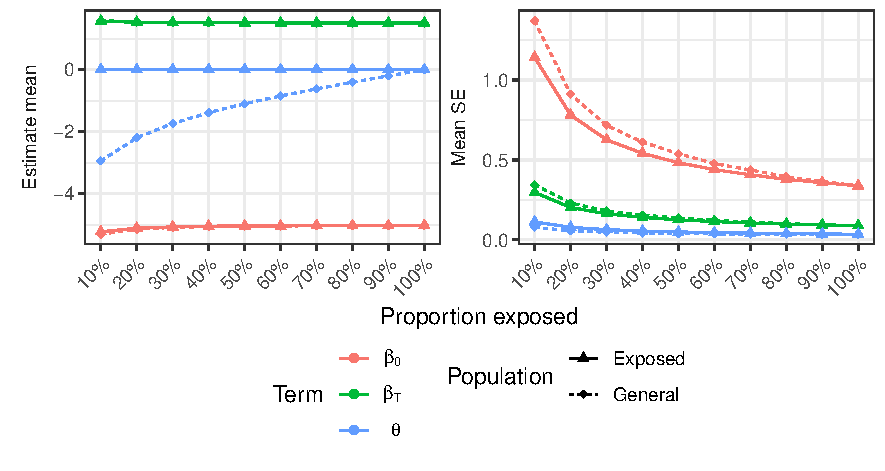
\includegraphics{sim-plot/plot2} 

}

\caption{The results of 10,000 simulations at each parameter combination. Points represent values at which simulations were performed. Points and lines are colored based on the estimated term they belong to. The solid lines and triangles show estimated mean (left panel) and mean standard error (right panel) of estimates obtained from fitting models to the exposed population (i.e.~unexposed excluded). The dashed lines and rhombi show the same for the general population (i.e.~unexposed included).}\label{fig:plot2}
\end{figure}

As expected, including the unexposed into the analysos has the effect of lowering the estimated baseline probability but has no appreciable effect on the expected estimates of the other parameters.

Including the unexposed into the anlalysis also has the effect of increasing the expected standard errors of the \(\beta\) parameters (especially the intercept \(\beta_0\)) by 5-10\% when the exposed proportion is less then 50\%.

\hypertarget{using-household-infection-as-an-indicator-of-exposure}{%
\section{Using household infection as an indicator of exposure}\label{using-household-infection-as-an-indicator-of-exposure}}

One way to distinguish between the exposed and the unexposed populations is to use infection status within the household. If there is at least one infection in a household, all of its members are assumed to have been exposed. If there are no infections in a household, none of its members are assumed to have been exposed.

However, there are likely to be households with memebers who were exposed but where nobody got infected. These households would be excluded from the analysis which may create problems for the validity of the estimates.

To investigate this, I simulated 10,000 observations from the same model as in Section \ref{se} except now everyone was assigned to a hoousehold. Each household had 4 subjects. The entire household was either exposed or unexposed according to the specified (expected) proportion. There was no random effect associated with being in a household. The results of 10,000 simulations at each value of proportion (of households) exposed are in Figure \ref{fig:plot3}.



\begin{figure}

{\centering 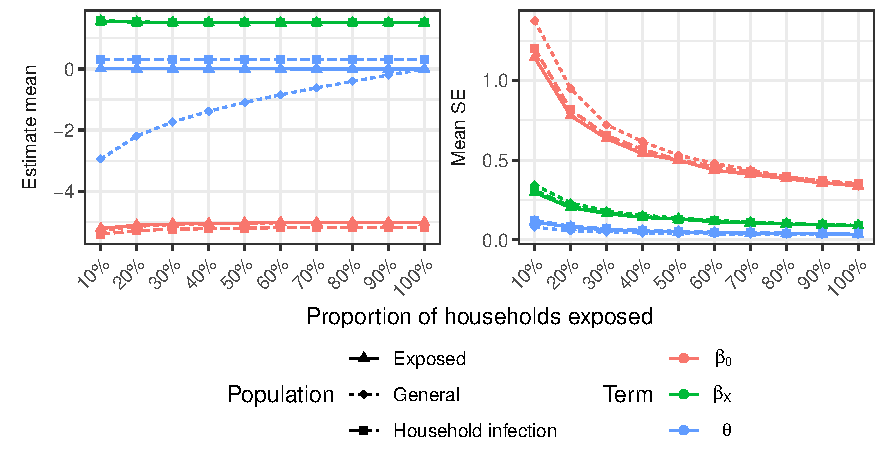
\includegraphics{sim-plot/plot3} 

}

\caption{The results of 10,000 simulations at each parameter combination. Points represent values at which simulations were performed. Points and lines are colored based on the estimated term they belong to. The solid lines and triangles show estimated mean (left panel) and mean standard error (right panel) of estimates obtained from fitting models to the exposed population (i.e.~unexposed excluded). The dashed lines and rhombi show the same for the general population (i.e.~unexposed included). The dash-dotted lines and squares show the same for the population with at least one infection in the household.}\label{fig:plot3}
\end{figure}

Using household infection as a measure of exposure appears to not introduce any notable bias in the estimates. The expected standard errors from this sample are similar to those that would have been obtained if the true infection status was known and everyone who was truly exposed was included into the analysis.

\hypertarget{conclusion}{%
\section{Conclusion}\label{conclusion}}

Including the unexposed into the analysis offers no benefits and has the detriment of increasing estimate error (despite the fact that there is more data with the unexposed included). If there is a good way to isolate the unexposed subjects in the analysis, those observations should be excluded. Household infection appears to be a reasonable measure of exposure despite the fact that some exposed households will likely be excluded.

\end{document}
